

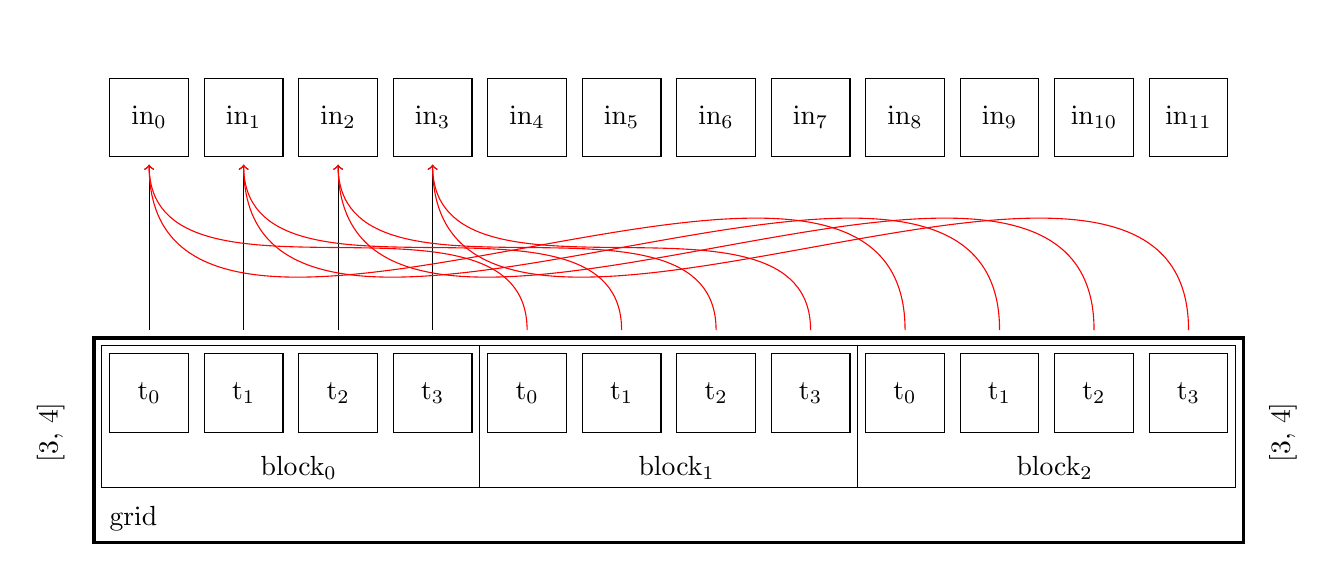
\begin{tikzpicture}[]


%%% DEFINITIONS %%%%%%%%%%%%%%%%%%%%%%%%%%%%%%%%%%%%%%%%%%%%%%%%%%%%%%%%%%%%%


% https://associatie.kuleuven.be/huisstijl/kleuren
\definecolor{blue1}{RGB}{82,189,236}
\definecolor{blue2}{RGB}{0,64,122}
\definecolor{blue3}{RGB}{31,171,231}
\definecolor{blue4}{RGB}{29,141,176}
\definecolor{blue5}{RGB}{17,110,138}
\definecolor{orange1}{RGB}{221,138,46}


\def\SignalY{2}
% \def\GridOneY{0}
\def\GridOneY{-1.5}
\def\GridTwoY{-3}
\def\MultiplierX{1.2}

\def\SquareSize{1}

\def\ThPoolCenterTwoX{2}
\def\ThPoolCenterTwoY{0}

\def\NumOfSamples{12}

\def\BlockDimX{4}


%%% DRAWING %%%%%%%%%%%%%%%%%%%%%%%%%%%%%%%%%%%%%%%%%%%%%%%%%%%%%%%%%%%%%%%%%



\foreach \x in {0,...,11} {
    \draw[black] (\x * \MultiplierX, \SignalY) rectangle ++ (\SquareSize, \SquareSize);
    \node at (\x * \MultiplierX + \SquareSize/2, \SignalY + \SquareSize/2) {in$_{\x}$};
}


\foreach \x in {0,...,11} {
    \draw[black] (\x * \MultiplierX, \GridOneY) rectangle ++ (\SquareSize, \SquareSize);
}

\foreach \x in {0,...,3} {
    \node at (\x * \MultiplierX + \SquareSize/2, \GridOneY + \SquareSize/2) {t$_{\x}$};
    \draw[<-] (\x * \MultiplierX + \SquareSize/2, \SignalY - 0.1) -- (\x * \MultiplierX + \SquareSize/2, \GridOneY + \SquareSize + 0.3);
}

\foreach \x in {0,...,3} {
    \node at (\x * \MultiplierX + \SquareSize/2 + \SquareSize * \MultiplierX * 4, \GridOneY + \SquareSize/2) {t$_{\x}$};
    \draw[red, <-] (\x * \MultiplierX + \SquareSize/2, \SignalY - 0.1) to [out=-90, in=90] (\x * \MultiplierX + \SquareSize/2 + \SquareSize * \MultiplierX * 4, \GridOneY + \SquareSize + 0.3);
    % \draw[red, <-] (\x * \MultiplierX + \SquareSize/2, \SignalY - 0.1) -- (\x * \MultiplierX + \SquareSize/2 + \SquareSize * \MultiplierX * 4, \GridOneY + \SquareSize + 0.3);
}

\foreach \x in {0,...,3} {
    \node at (\x * \MultiplierX + \SquareSize/2 + \SquareSize * \MultiplierX * 8, \GridOneY + \SquareSize/2) {t$_{\x}$};
    \draw[red, <-] (\x * \MultiplierX + \SquareSize/2, \SignalY - 0.1) to [out=-90, in=90] (\x * \MultiplierX + \SquareSize/2 + \SquareSize * \MultiplierX * 8, \GridOneY + \SquareSize + 0.3);
    % \draw[red, <-] (\x * \MultiplierX + \SquareSize/2, \SignalY - 0.1) -- (\x * \MultiplierX + \SquareSize/2 + \SquareSize * \MultiplierX * 8, \GridOneY + \SquareSize + 0.3);
}


\foreach \x in {0,...,2} {
    \draw[black] (-0.1 + \x * \MultiplierX * \BlockDimX, \GridOneY - 0.1 - 0.6) rectangle ++ (\SquareSize * \MultiplierX * \BlockDimX, \SquareSize + 0.2 + 0.6);
    \node at ({(\x + 0.5) * \MultiplierX * \BlockDimX}, \GridOneY - 0.45) {block$_\x$};
}


\draw[black, very thick] (-0.2, \GridOneY - 0.2 - 0.6 - 0.6) rectangle ++ (\SquareSize * \MultiplierX * \NumOfSamples + 0.2, \SquareSize + 0.4 + 0.6 + 0.6);
\node at (0.3, \GridOneY-1.1) {grid};

\node[rotate=90] at (-0.75, \GridOneY) {[3, 4]};
\node[rotate=90] at (\SquareSize * \MultiplierX * \NumOfSamples + 0.5, \GridOneY) {[3, 4]};


\end{tikzpicture}